\documentclass[../poma-notes.tex]{subfiles}

\begin{document}

本章基于黎曼积分的定义,该定义明确的取决于实线的层次结构。因此首先我们将探讨区间内实值函数的积分,然后再是复数与向量函数的积分,
而非区间积分将会在第十与十一章进行探讨。

\subsection*{Definition and Existence of the Integral}

\begin{definition}
  Let $[a,b]$ be a given interval. By a \textit{partition} $P$ of $[a,b]$ we mean a finite set of points
  $x_0, x_1, \dots, x_n$, where
  \[
    a = x_0 \le x_1 \le \cdots \le x_{n-1} \le x_n = b.
  \]

  We write
  \[
    \delta x_i = x_i - x_{i-1} \qquad (i=1,\dots,n).
  \]
  Now suppose $f$ is a bounded real function defined on $[a,b]$. Corresponding to each partition $P$ of
  $[a,b]$ we put
  \begin{align*}
    \begin{split}
      M_i &= \sup f(x) \qquad (x_{i-1} \le x \le x_i), \\
      m_i &= \inf f(x) \qquad (x_{i-1} \le x \le x_i), \\
      U(P,f) &= \sum_{i=1}^{n} M_i \delta x_i, \\
      L(P,f) &= \sum_{i=1}^{n} m_i \delta x_i,
    \end{split}
  \end{align*}
  and finally
  \begin{equation}
    \tint_{a}^{b} f \,dx = \inf\, U(P, f),
  \end{equation}
  \begin{equation}
    \bint_{a}^{b} f \,dx = \sup\, L(P, f),
  \end{equation}
  where the inf and the sup are taken over all partitions $P$ of $[a,b]$. The left members of (1) and (2)
  are called the \textit{upper} and \textit{lower Riemann integrals} of $f$ over $[a,b]$, respectively.

  If the upper and lower integrals are equal, we say that $f$ is \textit{Riemann-integrable} on $[a,b]$,
  we write $f \in \mathscr{R}$ (that is, $\mathscr{R}$ denotes the set of Riemann-integrable functions),
  and we denote the common value of (1) and (2) by
  \begin{equation}
    \int_{a}^{b}f\,dx,
  \end{equation}
  or by
  \begin{equation}
    \int_{a}^{b}f(x)\,dx.
  \end{equation}

  This is the \textit{Riemann integral} of $f$ over $[a,b]$. Since $f$ is bounded, there exist two numbers,
  $m$ and $M$, such that
  \[
    m \le f(x) \le M \qquad (a \le x \le b).
  \]
  Hence, for every $P$,
  \[
    m(b-a) \le L(P, f) \le U(P, f) \le M(b-a),
  \]
  so that the numbers $L(P, f)$ and $U(P, f)$ form a bounded set. This shows that \textit{the upper and lower
    integrals are defined for every} bounded function $f$. The question of their equality, and hence the question
  of the integrability of $f$, is a more delicate one. Instead of investigating it separately for the Riemann
  integral, we shall immediately consider a more general situation.
\end{definition}

\begin{anote}
  \begin{enumerate}
    \item \textbf{Partition}: $[a, b]$ 区间的分割。
    \item \textbf{Sub-interval}:每个 $[x_i, x_{i+1}]$ 即 partition 的 \textbf{子区间}。
    \item \textbf{Mesh}/\textbf{Norm}:一个 partition 的 mesh 或 norm,即最长的那个子区间 $\max(x_{i+1} - x_i),\ i\in[0, n-1]$。
    \item \textbf{Tagged partition}:取样分割,$P(x,t)$ 指在进行分割 $a = x_0 < x_1 < x_2 < \dots < x_n = b$ 后,
          与每一个子区间中 $[x_i,x_{i+1}]$ 取出一点 $x_i \le t_i \le x_{i+1}$。
    \item \textbf{Refinement}:精细化分割。假设两个分区 $P(x,t)$ 与 $Q(y,s)$ 皆为区间 $[a,b]$ 的分区。对于每个整数 $i,\ i\in[0,n]$,
          存在一个整数 $r(i)$ 满足 $x_i = y_{r(i)}$,以及对于某 $j,\ j\in[r(i),r(i+1)]$ 满足 $t_i = s_j$,那么我们可以将 $Q(y,s)$
          称为 $P(x,t)$ 的精细化分割。简言之,$Q(y,s)$ 是在 $P(x,t)$ 的基础上添加一些分点和标记。那么可以在此区间的所有采样分割中定义一个
          \href{https://en.wikipedia.org/wiki/Partially_ordered_set}{偏序关系 partially ordered set},称作\say{精细}。
    \item \textbf{Riemann sum}:黎曼和。令 $f$ 为定义在区间 $[a,b]$ 上的实值函数,$f$ 的黎曼和取决于取样分割 $x_0,\dots,x_n$,
          $t_0,\dots,t_{n-1}$:
          \[
            \sum_{i=0}^{n-1}f(t_i)(x_{i+1}-x_i)
          \]
          其中 $f(t_i)$ 视作高度,$x_{i+1} - x_i$ 视作宽度,而黎曼和则是所有带符号的矩形区域之和。
    \item \textbf{Upper \& lower Riemann Sums}:上黎曼和 $U(P,f) = \sum_{i=1}^{n} M_i \delta x_i$ 与下黎曼和
          $L(P,f) = \sum_{i=1}^{n} m_i \delta x_i$,详见下图。
    \item \textbf{Upper \& lower Riemann integrals}:上黎曼积分与下黎曼积分。严格定义如下:$S$ 是函数 $f$ 在闭区间 $[a,b]$ 上的黎曼积分,
          当且仅当对于任意的 $\varepsilon > 0$,都存在 $\delta > 0$,使得对于任意的取样分割 $x_0,\dots,x_n$,$t_0,\dots,t_{n-1}$,
          只要它的子区间长度最大值 $\lambda \le \delta$,就有
          \[
            \biggl| \sum_{i=0}^{n-1} f(t_i)(x_{i+1} - x_i) - S \biggr| < \varepsilon
          \]
    \item \textbf{Riemann-integrable}:黎曼可积。对于一个函数 $f$,如果在闭区间 $[a,b]$ 上,无论怎样进行取样分割,
          只要它的子区间长度最大值足够小,函数 $f$ 的黎曼和都会趋向于一个确定的值,那么 $f$ 在闭区间 $[a,b]$ 上的黎曼积分存在,
          并且定义为黎曼和的极限,这时候称函数 $f$ 为黎曼可积的(上下黎曼积分相等时,$f$ 在区间 $[a,b]$ 上黎曼可积)。然而这个定义的缺陷是没有
          可操作性,因为要检验所有 $\lambda \le \delta$ 的取样分割是很难做到的(接下来的定义更具有普适性)。
  \end{enumerate}
\end{anote}


\begin{figure}[htp]
  \centering
  \subfloat[$n=10$]{
    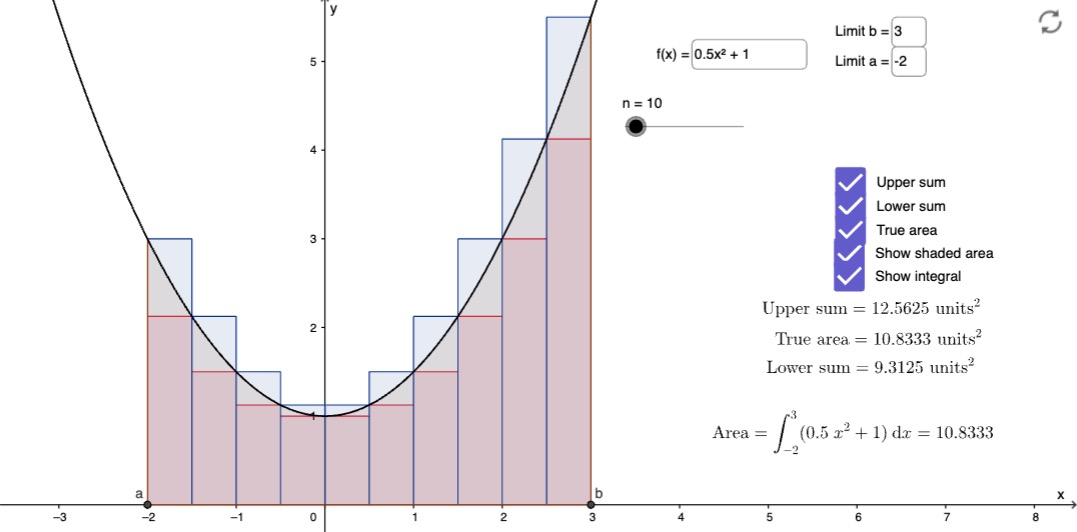
\includegraphics[width=0.4\textwidth]{\subfix{../images/UpperAndLowerRiemannSums1.png}}
  }
  \hfill
  \subfloat[$n=50$]{
    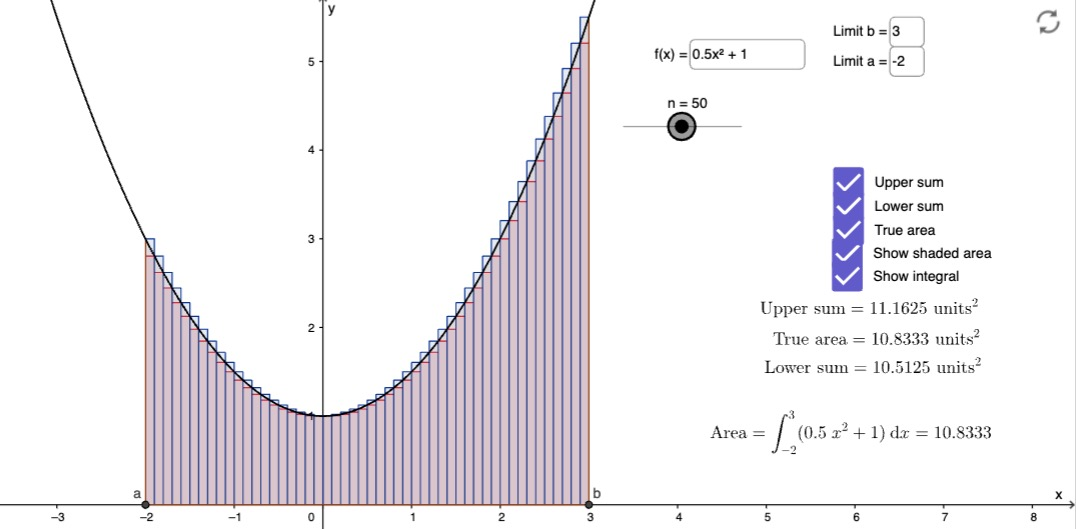
\includegraphics[width=0.4\textwidth]{\subfix{../images/UpperAndLowerRiemannSums2.png}}
  }
  \caption*{Upper and lower Riemann sums}
\end{figure}

% TODO

\end{document}
